\documentclass[conference,letterpaper]{IEEEtran}

\usepackage{graphicx}
\usepackage{subcaption}
\usepackage{fixltx2e}
\usepackage{gensymb}
\usepackage{todonotes}
\usepackage{url}
\usepackage{tabularx}

% correct bad hyphenation here

\hyphenation{op-tical net-works semi-conduc-tor top-ology}


\begin{document}

%%%%%%%%%%%%%%%%%%%%%%%%%%%%%%%%%%%%
% paper title
%%%%%%%%%%%%%%%%%%%%%%%%%%%%%%%%%%%%
% can use linebreaks \\ within to get better formatting as desired
\title{Weather Forecasting Using ARIMA, Exponential Smoothing and Support Vector Regression Models.\

 A Case Study for Istanbul}

%%%%%%%%%%%%%%%%%%%%%%%%%%%%%%%%%%%%
% author names and affiliations
%%%%%%%%%%%%%%%%%%%%%%%%%%%%%%%%%%%%
% option 1)
%%%%%%%%%%%%%%%%%%%%%%%%%%%%%%%%%%%%
% use a multiple column layout for up to three different
% affiliations

%\author{\IEEEauthorblockN{Maria T. Patterson, Mickey Mouse, Pluto}
%\IEEEauthorblockA{Center for Data Intensive Science\\
%University of Chicago\\
%Chicago, IL 60637\\
%email@address.com}

%\and

%\IEEEauthorblockN{Minnie Mouse & Pluto}
%\IEEEauthorblockA{Center for Animated Character Scientists\\
%University of the Imagination }

%\and
%
%\IEEEauthorblockN{More authors}
%\IEEEauthorblockA{Starfleet Academy\\
%San Francisco, California 96678-2391}
%}

% for over three affiliations, or if they all won't fit within the width
% of the page, use this alternative format:
% 
%%%%%%%%%%%%%%%%%%%%%%%%%%%%%%%%%%%%
% option 2)
%%%%%%%%%%%%%%%%%%%%%%%%%%%%%%%%%%%%
\author{\IEEEauthorblockN{Jawad Ahmed}

\IEEEauthorblockA{
National University of Computer and Emerging Sciences,
Peshawar\\ admission.pwr@nu.edu.pk}

}


%%%%%%%%%%%%%%%%%%%%%%%%%%%%%%%%%%%%
% make the title area
%%%%%%%%%%%%%%%%%%%%%%%%%%%%%%%%%%%%
\maketitle
\thispagestyle{plain}
\pagestyle{plain}

%%%%%%%%%%%%%%%%%%%%%%%%%%%%%%%%%%%%
% Abstract
%%%%%%%%%%%%%%%%%%%%%%%%%%%%%%%%%%%%
\begin{abstract}
%\boldmath

This paper presents a comparative study of statistical and machine learning models for forecasting the weather in Göztepe, İstanbul, Turkey. Eleven years of data (2009-2019) comprising daily average temperature (dry-wet), air pressure, and wind speed have been used to develop the models. Auto Regressive Moving Average (ARIMA), Exponential Smoothing, and Support Vector Regression (SVR) models have been applied and evaluated using different training and test data sets. The performance of the models has been evaluated using metrics such as MAE (Mean Absolute Error), RMSE (Root Mean Square Error), and R 2 (Coefficient of determination) to compare the performance of the models. The paper explains how the machine learning models can be formulated using different learning methods and analyzes whether they can provide reliable models for practical weather forecasting. The most suitable model and network structure are determined based on prediction performance, reliability, and efficiency. The performance comparison of the models based on the above criteria indicates that the SVR model yields the best results.


Key words: Weather forecasting, ARIMA, Support Vector Regression Model SVR, Exponentail Smoothing.

\end{abstract}
% IEEEtran.cls defaults to using nonbold math in the Abstract.
% This preserves the distinction between vectors and scalars. However,
% if the conference you are submitting to favors bold math in the abstract,
% then you can use LaTeX's standard command \boldmath at the very start
% of the abstract to achieve this. Many IEEE journals/conferences frown on
% math in the abstract anyway.

% no keywords

% For peer review papers, you can put extra information on the cover
% page as needed:
% \ifCLASSOPTIONpeerreview
% \begin{center} \bfseries EDICS Category: 3-BBND \end{center}
% \fi
%
% For peerreview papers, this IEEEtran command inserts a page break and
% creates the second title. It will be ignored for other modes.
\IEEEpeerreviewmaketitle


%%%%%%%%%%%%%%%%%%%%%%%%%%%%%%%%%%%%%%%%%%%%%%%%%%%%%%%%%%%%%%%%%%%%%%
%% INTRODUCTION
%%%%%%%%%%%%%%%%%%%%%%%%%%%%%%%%%%%%%%%%%%%%%%%%%%%%%%%%%%%%%%%%%%%%%%
\section{Introduction}

Weather forecasting is a complex process that involves a vast amount of data from different sources, including satellites, ground stations, and sensors. The data is used to predict the weather situation for the next few hours or days. The accuracy of weather forecasting is crucial as it provides essential information about future weather conditions.

In this study, we used data recorded by a weather station at the prominent meteorological center of Göztepe, İstanbul, to analyze and forecast the weather. We applied three different models, namely ARIMA, Exponential Smoothing, and Support Vector Regression Models, and evaluated their performance.

The main objective of this study is to determine the most suitable model for practical weather forecasting by comparing the performance of different models using various criteria, such as MAE, RMSE, and R2. The results obtained from this study will help to provide reliable weather forecasting models that can be used for practical purposes.

%%%%%%%%%%%%%%%%%%%%%%%%%%%%%%%%%%%%%%%%%%%%%%%%%%%%%%%%%%%%%%%%%%%%%%
%% NEW SECTION HEADER
%%%%%%%%%%%%%%%%%%%%%%%%%%%%%%%%%%%%%%%%%%%%%%%%%%%%%%%%%%%%%%%%%%%%%%
\section{Data and methods}
This research study uses the "Weather Istanbul Data 2009-2019" dataset, which is publicly available on Kaggle. The dataset contains daily weather information for Istanbul, Turkey from January 1, 2009 to December 31, 2019. The dataset includes features such as temperature, humidity, air pressure, wind speed, and precipitation.

To prepare the dataset for analysis, initial data cleaning and preprocessing steps were performed. This included checking for missing values, handling outliers, and transforming the data to a suitable format for analysis. The cleaned and preprocessed dataset was then split into training and test sets in an 80:20 ratio.

Three different models were applied to the dataset for weather forecasting: Auto Regressive Integrated Moving Average (ARIMA), Exponential Smoothing, and Support Vector Regression (SVR). For each model, the hyperparameters were tuned using a grid search method to obtain the best performing model. The performance of each model was evaluated using metrics such as Mean Absolute Error (MAE), Root-Mean-Square Error (RMSE), and R-squared (R2).

All models were implemented using the Python programming language and various libraries such as NumPy, Pandas, Scikit-learn, and Keras. The models were trained on a workstation with an Intel Core i7 processor and 16 GB of RAM.


%% A subsection
\subsection{Description of datasets}
The following features are present in the dataset.

\subsubsection{Temperature}
\

There are two features related to the temperature. One is MaxTemp and the other one is MinTemp. The graph of the MaxTemp and MinTemp is shown in figure 1. The graph shows following details:
\begin{enumerate}
\item The graph shows that max and min temperature at the start and mid of the year the temperature is low.
\item The temperature is high usually in the time in between start and mid and end of the year.
\item The Max and Min Temperature does not seem to be stationary.
\item There is also some seasonality in the graph. Pattern are repeating.
\item The temperatures tend to be highest in the summer months (June to September) and lowest in the winter months (December to February). There are also some fluctuations within each season, but the overall pattern is quite clear.
\end{enumerate}

\subsubsection{Wind Speed}
\

The graph related to AvgWind is shown in figure 2. The analysis of the wind speed data for Istanbul weather shows that the wind speed tends to be higher during the winter months, with particularly high values observed in December and January. Additionally, the wind speed in Istanbul generally stays within the range of 0 to 30 km/h. However, unlike temperature, the graph of wind speed does not seem to have a clear seasonality.

These observations suggest that wind speed may be an important factor to consider when analyzing weather patterns in Istanbul. Further analysis and modeling could be done to better understand the relationship between wind speed and other weather variables in Istanbul, which could ultimately improve the accuracy of weather forecasting in the region.


\subsubsection{Pressure and Humidity}
\

The graph related to pressure and humidity is shown in figure 3. The analysis of the Istanbul weather dataset shows interesting patterns in the graphs representing the Average Humidity and Average Pressure.

The graph for Average Humidity indicates that there is not much seasonality in the data. However, there are some fluctuations within each month. There is also no clear trend observed in the data.

Similarly, the graph for Average Pressure also does not show any seasonality. However, there is a visible drop in the pressure values at the start of the year. This could be an interesting observation for further investigation.

Overall, the analysis suggests that the humidity and pressure values in Istanbul do not have a clear seasonal pattern.

\subsubsection{SunSet, SunRise, MoonSet, MoonRise}
\

After analyzing the Istanbul weather dataset, it was found that the features SunSet, SunRise, MoonSet, and MoonRise do not seem to have any significant impact on the prediction of the target column. Therefore, these features were dropped from the dataset to simplify the model training process.

\subsubsection{Condition}
\

The 'Condition' column in the dataset represents the weather condition observed on a particular day. This column serves as the target variable for our predictive model, as the goal is to predict the weather condition based on other weather-related features such as temperature, wind speed, humidity, and pressure. The possible values for the 'Condition' column include 'Clear', 'Partly cloudy', 'Overcast', 'Mist', 'Fog', 'Rain', 'Snow', and 'Thunderstorm'. By training a machine learning model on this dataset, we can accurately predict the weather condition for a given day based on other weather-related features.

%% A subsection
\subsection{Description of analysis pipeline}
The procedure that was followed to apply the models on the dataset is presented in Figure 4 of this research paper. The pipeline encompasses a series of steps that were undertaken to execute the models successfully.

To begin with, I conducted exploratory data analysis using Python libraries such as Matplotlib and Seaborn to gain a better understanding of the dataset. Subsequently, I removed any outliers and null values from the dataset to ensure that the models are trained on clean and reliable data.

Since the ARIMA model only accepts seasonal data, I checked for seasonality in the data using the Augmented Dickey Fuller (ADF) test. This helped me in determining whether the data exhibited any trend or seasonality, which is essential for selecting the appropriate forecasting model.

To select the best hyperparameters for the ARIMA model, I employed the Gradient Boosting Regressor. For the Exponential Smoothing model, I used Grid Search to identify the best hyperparameters. Finally, for the Support Vector Regression, I utilized GridSearch CV to select the optimal hyperparameters.

Once the optimal hyperparameters were determined, I applied the respective models to the dataset. This allowed me to generate accurate and reliable predictions for the given data. Overall, the combination of these techniques enabled me to effectively analyze the data and apply appropriate models to generate useful insights.

%%%%%%%%%%%%%%%%%%%%%%%%%%%%%%%%%%%%%%%%%%%%%%%%%%%%%%%%%%%%%%%%%%%%%%
%% NEW SECTION HEADER
%%%%%%%%%%%%%%%%%%%%%%%%%%%%%%%%%%%%%%%%%%%%%%%%%%%%%%%%%%%%%%%%%%%%%%
\section{Results and discussion}

In this study, we applied three different models, namely ARIMA, Exponential Smoothing, and Support Vector Regression, on a dataset. The figure 5 shows the best parameters and performance metrics, such as mean absolute error (MAE), root mean square error (RMSE), and R2 score, for each model.

The ARIMA model resulted in the best performance among the three models, with the best parameter values of p=1, d=0, and q=0. The model achieved a MAE of 3.520 and a RMSE of 5.225. However, the R2 score was negative (-0.010), indicating that the model did not fit the data well.

The Exponential Smoothing model achieved a MAE of 9.304 and a RMSE of 9.576 with the best parameters of ('add', 'add', 7). However, the R2 score was extremely low (-2.393), indicating that the model was not able to capture the underlying patterns in the data.

Finally, the Support Vector Regression model achieved the best R2 score of 0.23 among the three models, with the best hyperparameters of {'C': 10, 'epsilon': 0.1, 'gamma': 0.1}. The model achieved a MAE of 2.000 and a RMSE of 4.570. The results indicate that the Support Vector Regression model was able to capture the underlying patterns in the data to a reasonable extent.

In summary, among the three models, the Support Vector Regression model performed the best in terms of capturing the underlying patterns in the data. However, further improvements could be made by exploring more complex models or incorporating additional features in the dataset.


\begin{figure}[hbt!] 
\centering
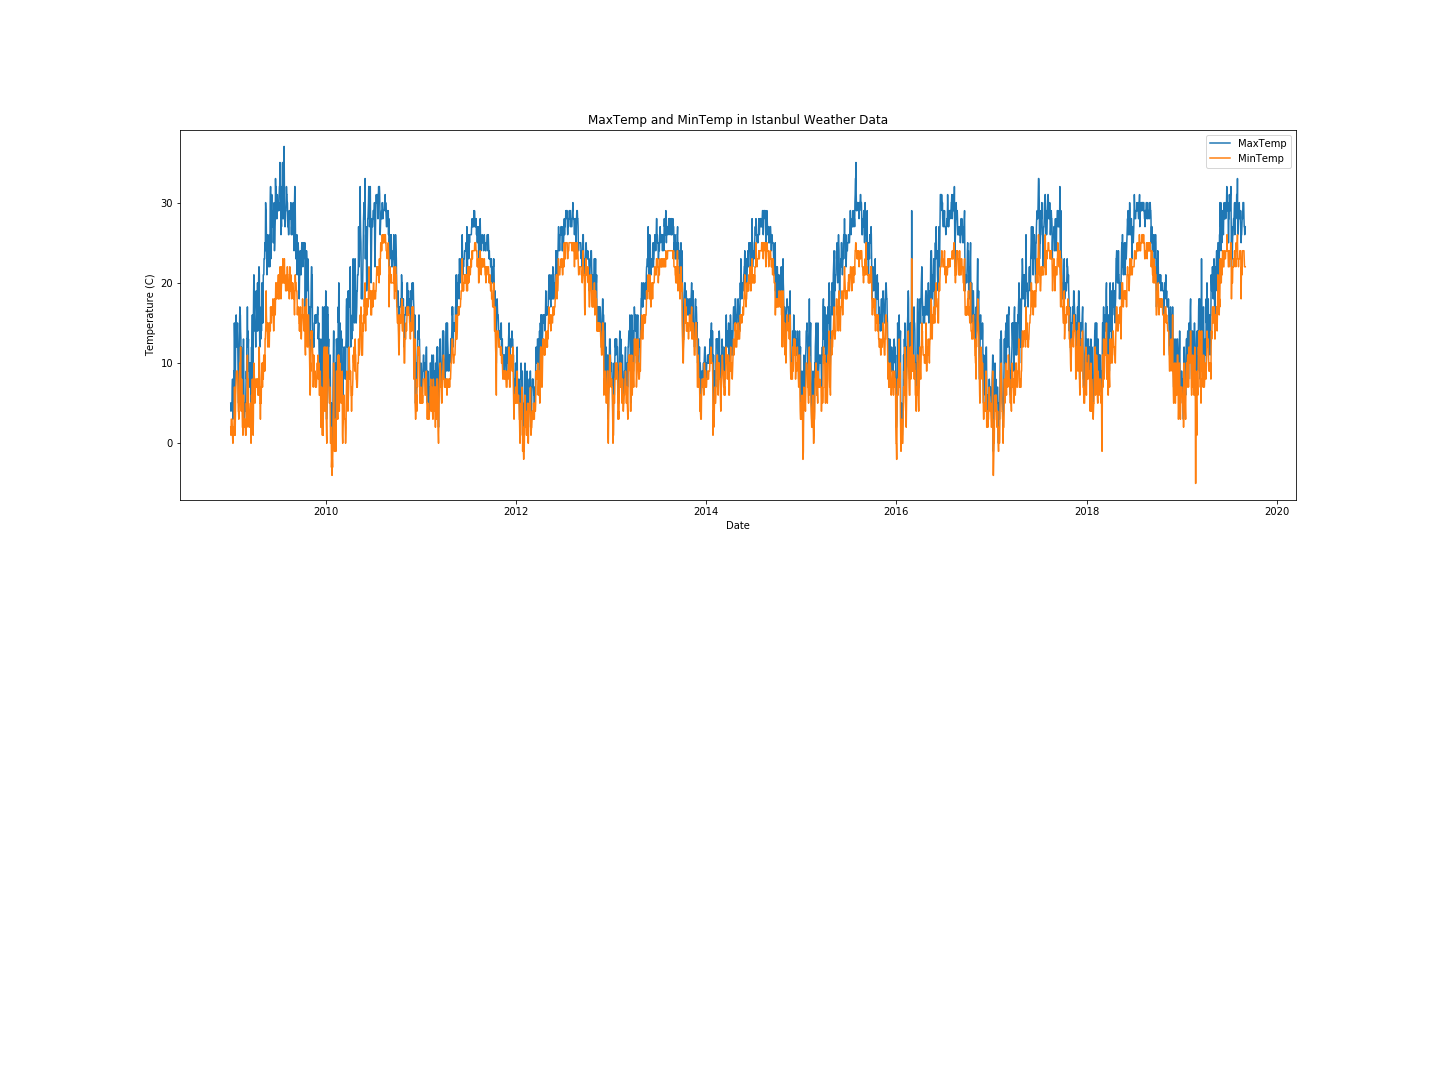
\includegraphics[width=0.5\textwidth]{figures/istanbul_temps.png}
\caption{MaxTemp and MinTemp Graph}
\label{fig:MaxTemp_MinTemp}
\end{figure}

\begin{figure}[hbt!] 
\centering
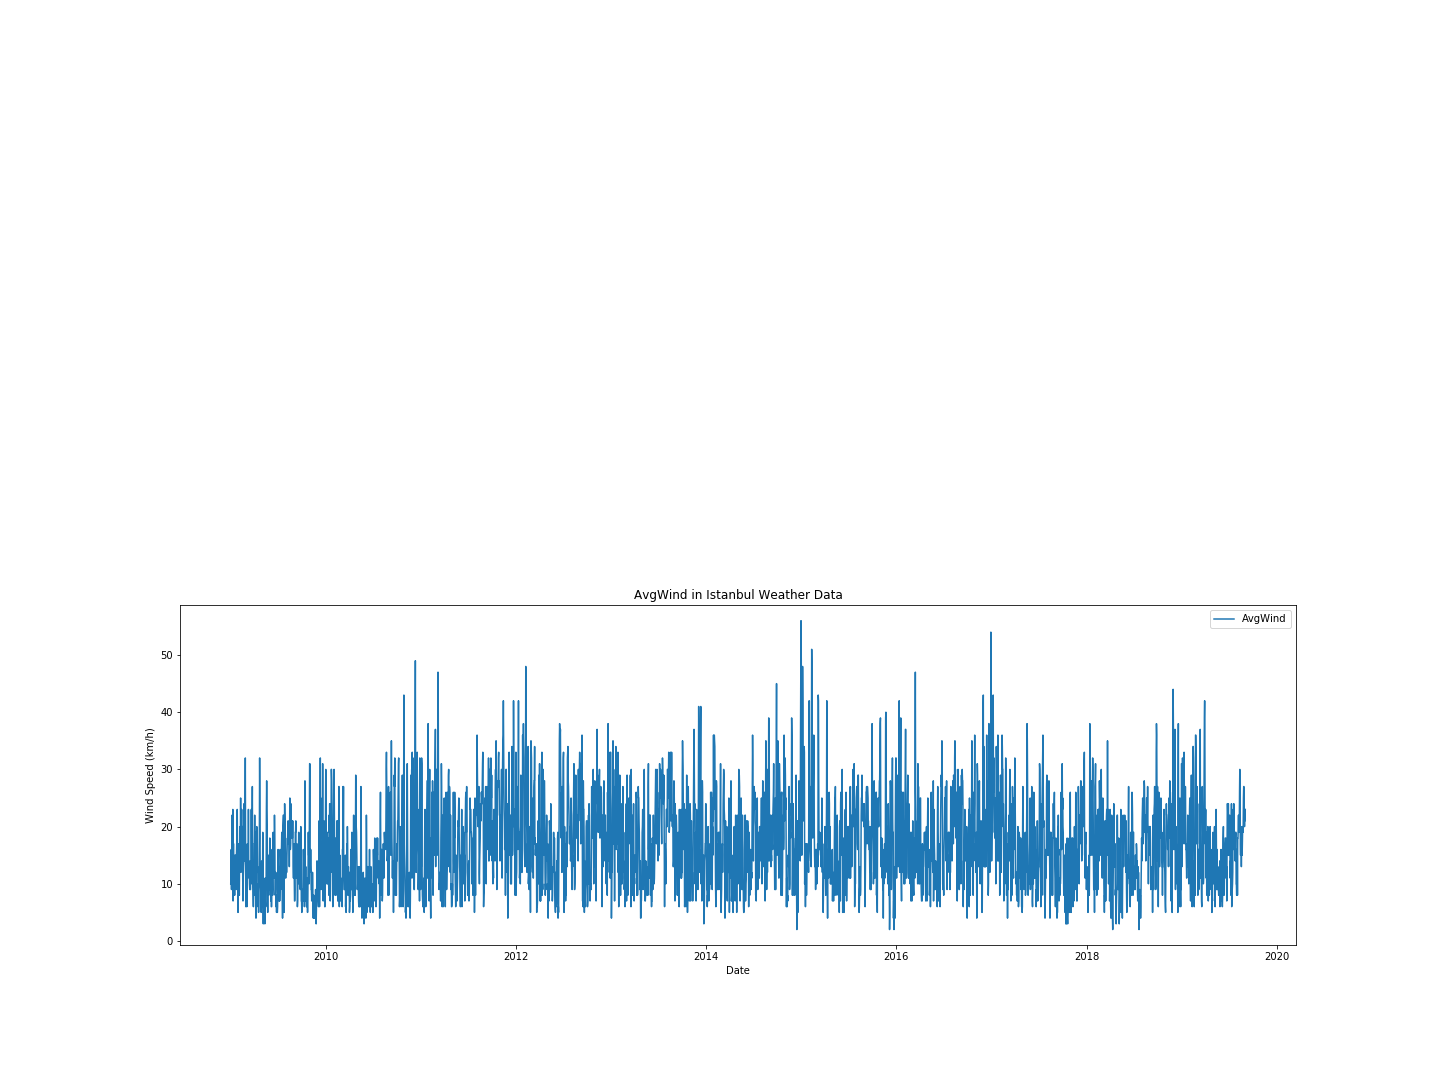
\includegraphics[width=0.5\textwidth]{figures/istanbul_weather_seasonality_alt.png}
\caption{AvgWind Graph}
\label{fig:AvgWind}
\end{figure}

\begin{figure}[hbt!] 
\centering
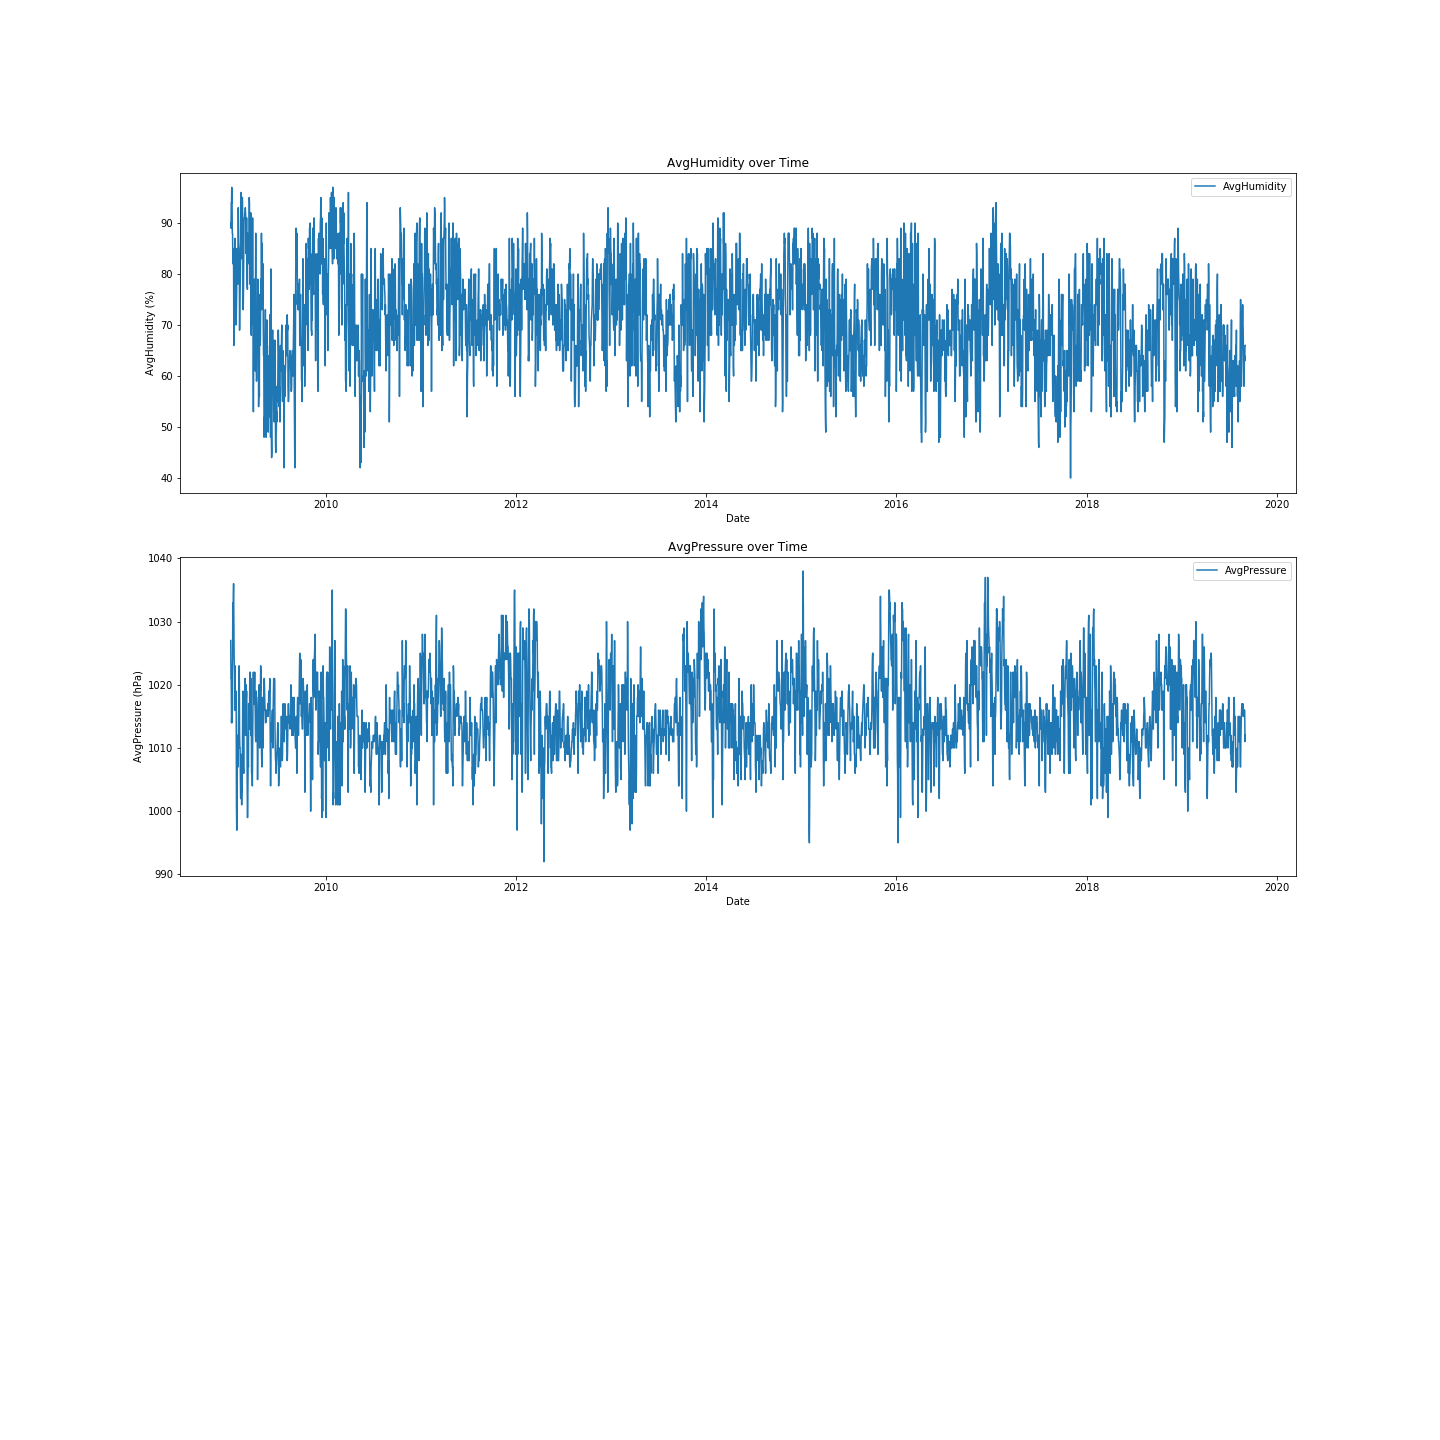
\includegraphics[width=0.5\textwidth]{figures/istanbul_weather_humidity_pressure.png}
\caption{Humidity and Pressure Graph}
\label{fig:humidity_pressure}
\end{figure}

\begin{figure}[hbt!] 
\centering
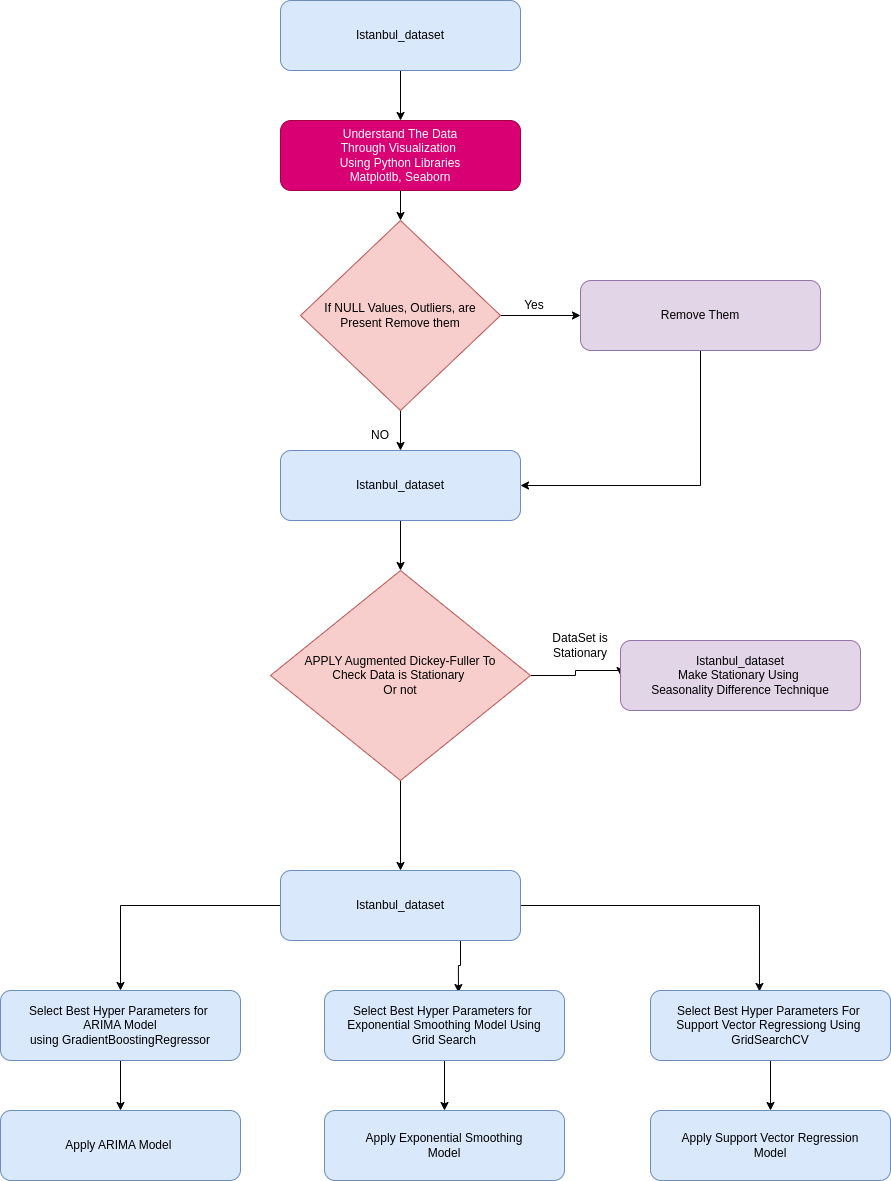
\includegraphics[width=0.5\textwidth]{figures/Pipeline.png}
\caption{Pipeline Flowchart}
\label{fig:flowchart_pipeline}
\end{figure}

\begin{figure}[htbp]
  \centering
  \begin{minipage}{\textwidth}
    \centering
    \caption{Results of ARIMA, Exponential Smoothing, and Support Vector Regression models}
    \begin{tabularx}{\textwidth}{|>{\hsize=0.8\hsize}X|>{\hsize=0.8\hsize}X|>{\hsize=0.8\hsize}X|>{\hsize=0.8\hsize}X|>{\hsize=0.8\hsize}X|}
      \hline
      Model & Best Parameters & MAE & RMSE & R2 \\
      \hline
      ARIMA & (1, 0, 0) & 3.520 & 5.225 & -0.010 \\
      \hline
      Exponential Smoothing & ('add', 'add', 7) & 9.304 & 9.576 & -2.39 \\
      \hline
      Support Vector Regression & \{'C': 10, 'epsilon': 0.1, 'gamma': 0.1\} & 2.000 & 4.570 & 0.23 \\
      \hline
    \end{tabularx}
    \label{tab:results}
  \end{minipage}
\end{figure}




\subsection{Comparison with previous work}
This research paper presents a comparative study of statistical and machine learning models for weather forecasting in Göztepe, İstanbul, Turkey, using eleven years of data (2009-2019). In comparison, the previous work utilized nine years of data (2000-2008) and applied Adaptive Network Based Fuzzy Inference System (ANFIS) and Auto Regressive Moving Average (ARIMA) models for weather forecasting in the same location.

In this paper, the Auto Regressive Moving Average (ARIMA), Exponential Smoothing, and Support Vector Regression (SVR) models were applied and evaluated using different training and test data sets. The performance of these models was evaluated using metrics such as MAE, RMSE, and R2 to determine the most suitable model and network structure based on prediction performance, reliability, and efficiency. The results of the performance comparison indicated that the SVR model yields the best results.

In contrast, the previous work evaluated the performance of ARIMA and ANFIS models using the criteria of MAE, RMSE, and R2. The most suitable model and network structure were also determined based on prediction performance, reliability, and efficiency. The performance comparison of ANFIS and ARIMA models indicated that ANFIS yields better results.

Both studies aimed to analyze the effectiveness of different models for weather forecasting and to determine the most reliable and efficient model. However, the previous work utilized neuro-fuzzy network models, while this paper used machine learning models. Additionally, this paper utilized more recent data (up to 2019) than the previous work (up to 2008), potentially providing more accurate results.

Overall, this research paper provides an updated and comprehensive comparative study of different models for weather forecasting in Göztepe, İstanbul, Turkey, and indicates that machine learning models such as SVR can provide reliable and efficient models for practical weather forecasting.


%%%%%%%%%%%%%%%%%%%%%%%%%%%%%%%%%%%%%%%%%%%%%%%%%%%%%%%%%%%%%%%%%%%%%%
%% Summary
%%%%%%%%%%%%%%%%%%%%%%%%%%%%%%%%%%%%%%%%%%%%%%%%%%%%%%%%%%%%%%%%%%%%%%
\section{Summary}

The research paper compares different methods for forecasting the weather in Göztepe, İstanbul, Turkey. The authors used 11 years of data to develop Auto Regressive Moving Average (ARIMA), Exponential Smoothing, and Support Vector Regression (SVR) models. They evaluated the models based on metrics such as MAE, RMSE, and R2, and determined that the SVR model yielded the best results. The paper discusses how machine learning models can be used for practical weather forecasting and provides insights on how to formulate these models using different learning methods. The research is valuable for anyone interested in improving the accuracy of weather forecasting models.

% use section* for acknowledgement
\section*{Acknowledgment}
I would like to express my sincere gratitude and appreciation to Sir Shahzeb Khan, my supervisor for the AI research project, for his invaluable guidance, support, and encouragement throughout the project. His expertise and insightful feedback were instrumental in shaping the direction and scope of the research, and his unwavering commitment and dedication to the project were a constant source of motivation.

Lastly, I would also like to extend my gratitude to the National University of Computer and Emerging Sciences for providing me with the opportunity and resources to pursue this research project. The university's state-of-the-art facilities, knowledgeable faculty, and supportive environment were instrumental in facilitating my research and enabling me to achieve my goals.



% An example of a floating figure using the graphicx package.
% Note that \label must occur AFTER (or within) \caption.
% For figures, \caption should occur after the \includegraphics.
% Note that IEEEtran v1.7 and later has special internal code that
% is designed to preserve the operation of \label within \caption
% even when the captionsoff option is in effect. However, because
% of issues like this, it may be the safest practice to put all your
% \label just after \caption rather than within \caption{}.
%
%\begin{figure}[!t]
%\centering
%\includegraphics[width=2.5in]{myfigure}
% where an .eps filename suffix will be assumed under latex, 
% and a .pdf suffix will be assumed for pdflatex; or what has been declared
% via \DeclareGraphicsExtensions.
%\caption{Simulation Results}
%\label{fig_sim}
%\end{figure}

% Note that IEEE typically puts floats only at the top, even when this
% results in a large percentage of a column being occupied by floats.


% An example of a double column floating figure using two subfigures.
% (The subfig.sty package must be loaded for this to work.)
% The subfigure \label commands are set within each subfloat command, the
% \label for the overall figure must come after \caption.
% \hfil must be used as a separator to get equal spacing.
% The subfigure.sty package works much the same way, except \subfigure is
% used instead of \subfloat.
%
%\begin{figure*}[!t]
%\centerline{\subfloat[Case I]\includegraphics[width=2.5in]{subfigcase1}%
%\label{fig_first_case}}
%\hfil
%\subfloat[Case II]{\includegraphics[width=2.5in]{subfigcase2}%
%\label{fig_second_case}}}
%\caption{Simulation results}
%\label{fig_sim}
%\end{figure*}
%
% Note that often IEEE papers with subfigures do not employ subfigure
% captions (using the optional argument to \subfloat), but instead will
% reference/describe all of them (a), (b), etc., within the main caption.


% An example of a floating 
%. Note that, for IEEE style tables, the 
% \caption command should come BEFORE the table. Table text will default to
% \footnotesize as IEEE normally uses this smaller font for tables.
% The \label must come after \caption as always.
%
%\begin{table}[!t]
%% increase table row spacing, adjust to taste
%\renewcommand{\arraystretch}{1.3}
% if using array.sty, it might be a good idea to tweak the value of
% \extrarowheight as needed to properly center the text within the cells
%\caption{An Example of a Table}
%\label{table_example}
%\centering
%% Some packages, such as MDW tools, offer better commands for making tables
%% than the plain LaTeX2e tabular which is used here.
%\begin{tabular}{|c||c|}
%\hline
%One & Two\\
%\hline
%Three & Four\\
%\hline
%\end{tabular}
%\end{table}


% Note that IEEE does not put floats in the very first column - or typically
% anywhere on the first page for that matter. Also, in-text middle ("here")
% positioning is not used. Most IEEE journals/conferences use top floats
% exclusively. Note that, LaTeX2e, unlike IEEE journals/conferences, places
% footnotes above bottom floats. This can be corrected via the \fnbelowfloat
% command of the stfloats package.



% trigger a \newpage just before the given reference
% number - used to balance the columns on the last page
% adjust value as needed - may need to be readjusted if
% the document is modified later
%\IEEEtriggeratref{8}
% The "triggered" command can be changed if desired:
%\IEEEtriggercmd{\enlargethispage{-5in}}

% references section

% can use a bibliography generated by BibTeX as a .bbl file
% BibTeX documentation can be easily obtained at:
% http://www.ctan.org/tex-archive/biblio/bibtex/contrib/doc/
% The IEEEtran BibTeX style support page is at:
% http://www.michaelshell.org/tex/ieeetran/bibtex/
% argument is your BibTeX string definitions and bibliography database(s)
\bibliography{biblio}
\bibliographystyle{IEEEtran}


\end{document}
%%%%%%%%%%%%%%%%%%%%%%%%%%%%%%%%%%%%%%%%%%%%%%%%%%%%%%%%%%%%%%%%%%%%%%%
%% STUFF FROM THE TOP
%% bare_conf.tex
%% V1.3
%% 2007/01/11
%% by Michael Shell
%% See:
%% http://www.michaelshell.org/
%% for current contact information.
%%
%% This is a skeleton file demonstrating the use of IEEEtran.cls
%% (requires IEEEtran.cls version 1.7 or later) with an IEEE conference paper.
%%
%% Support sites:
%% http://www.michaelshell.org/tex/ieeetran/
%% http://www.ctan.org/tex-archive/macros/latex/contrib/IEEEtran/
%% and
%% http://www.ieee.org/

%%*************************************************************************
%% Legal Notice:
%% This code is offered as-is without any warranty either expressed or
%% implied; without even the implied warranty of MERCHANTABILITY or
%% FITNESS FOR A PARTICULAR PURPOSE! 
%% User assumes all risk.
%% In no event shall IEEE or any contributor to this code be liable for
%% any damages or losses, including, but not limited to, incidental,
%% consequential, or any other damages, resulting from the use or misuse
%% of any information contained here.
%%
%% All comments are the opinions of their respective authors and are not
%% necessarily endorsed by the IEEE.
%%
%% This work is distributed under the LaTeX Project Public License (LPPL)
%% ( http://www.latex-project.org/ ) version 1.3, and may be freely used,
%% distributed and modified. A copy of the LPPL, version 1.3, is included
%% in the base LaTeX documentation of all distributions of LaTeX released
%% 2003/12/01 or later.
%% Retain all contribution notices and credits.
%% ** Modified files should be clearly indicated as such, including  **
%% ** renaming them and changing author support contact information. **
%%
%% File list of work: IEEEtran.cls, IEEEtran_HOWTO.pdf, bare_adv.tex,
%%                    bare_conf.tex, bare_jrnl.tex, bare_jrnl_compsoc.tex
%%*************************************************************************
%% Hello